%
% File eacl2009.tex
%
% Contact  oflazer@gmail.com or das@ling.uni-potsdam.de
%%

%% Based on the style files for EACL 2006 by 
%%e.agirre@ehu.es or Sergi.Balari@uab.es
%% and that of ACL 08 by Joakim Nivre and Noah Smith

\documentclass[11pt]{article}
\usepackage{eacl2009}
\usepackage{times}
\usepackage{url}
\usepackage{latexsym}
\usepackage[icelandic]{babel}
\usepackage[T1]{fontenc}
\usepackage[utf8]{inputenc}
\usepackage{graphicx}

%\setlength\titlebox{6.5cm}    % You can expand the title box if you
% really have to

\title{Rýnir}

\author{Arnór Barkarson\\
  Reykjavík University\\
  Reykjavík, Iceland\\
  {\tt arnorbarkar@ru.is}  \And  
  Ragnar Lárus Sigurðsson\\
  Reykjavík University\\
  Reykjavík, Iceland\\
  {\tt  ragnarls08@ru.is}\\ \And 
  Þórður Arnarsson\\
  Reykjavík University\\
  Reykjavík, Iceland\\
  {\tt  thordura08@ru.is}  \And 
  Gunnar Sveinsson\\
  Reykjavík University\\
  Reykjavík, Iceland\\
  {\tt  gunnarsve06@ru.is} 
}



\date{}

\begin{document}
\maketitle


\section{Summary}
\section{Introduction}
\section{Body}

\subsection{Bollinger bands}
\label{sec:third}

Bollinger bönd eru upprunalega þróuð sem greiningartól á þróun verðbréfaverða. Síðan þá hefur þessari aðferð verið beitt á ýmis
vandamál með misgóðum niðurstöðum. \\

Bollinger bönd samanstanda af
\begin{itemize}
  \item Miðband, N-lotu einfalt hlaupandi meðaltal (HM).
  \item Efra band, N-lotu staðalfrávik margfaldað með K, fyrir ofan miðbandið (HM + K$\sigma$).
  \item Neðra band, N-lotu staðalfrávik margfaldað með K, fyrir neðan miðbandið (HM - K$\sigma$).
\end{itemize}

Bollinger böndin nýtast því vel til þess að greina hvar í tímalínu óeðlileg hækkun eða lækkun á sér stað.



...

Útfærslan okkar byggist á því að keyra ítranir af Bollinger böndum á tímalínu með mismunandi gluggastærð, þar sem gluggastærðin er að hluta til ákvörðuð
af stærð tímalínunnar. Hverri ítrun er síðan gefið ákveðið vægi miðað við gluggastærð hennar, væginu er hagað þannig að 100\% vægi skiptist niður á ítranirnar.

...

\begin{figure}
  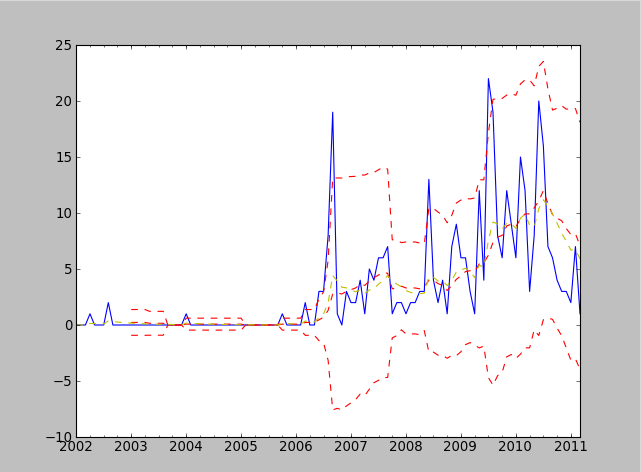
\includegraphics[width=.15\textwidth]{bollinger.jpg}
  %\caption{Bollinger bands\label{fig:first}}
\end{figure}




\section{Conclusion}
\section{Abstract}

 



\end{document}
